\chapter*{\vspace*{2ex}\emph{Preface}}
\slatexignorecurrentfile

This book started from the premise that Computer Science should be taught as a liberal art, not an industrial skill.  I had the privilege of taking 6.001 from Gerry Sussman when I was a first year student at MIT, and that course awakened me to the power and beauty of computing, and inspired me to pursue a career as a teacher and researcher in Computer Science.  When I arrived as a new faculty member at the University of Virginia in 1999, I was distraught to discover that the introductory computing courses focused on teaching industrial skills, and with so much of the course time devoted to explaining the technical complexities of using bloated industrial languages like C++ and Java, there was very little, if any, time left to get across the core intellectual ideas that are the essence of computing and the reason everyone should learn it.  

With the help of a University Teaching Fellowship and National Science Foundation grants, I developed a new introductory computer science course, targeted especially to students in the College of Arts \& Sciences.  This course was first offered in Spring 2002, with the help of an extraordinary group of Assistant Coaches.  Because of some unreasonable assumptions in the first assignment, half the students quickly dropped the course, but a small, intrepid, group of pioneering students persisted, and it is thanks to their efforts that this book exists.  That course, and the next several offerings, used Abelson \& Sussman's outstanding \emph{Structure and Interpretation of Computer Programs} (SICP) textbook along with Douglas Hofstadter's \emph{\Godel, Escher, Bach: An Eternal Golden Braid}.\index{general}{MIT}\index{people}{Sussman, Gerald}  

{\centering
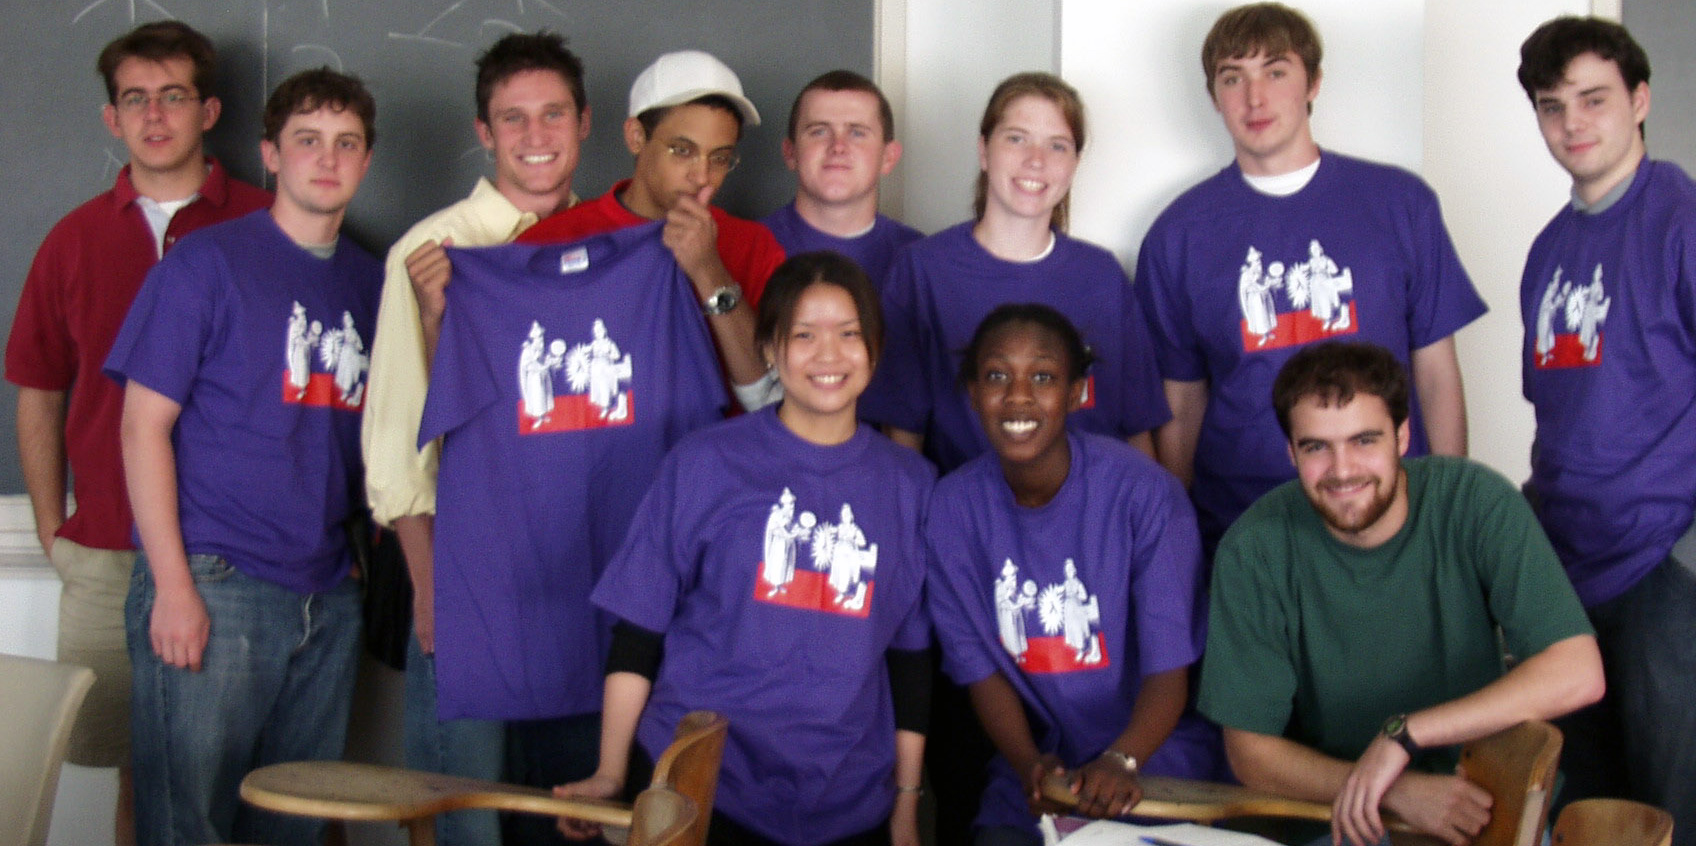
\includegraphics[width=4.0in]{images/cs200-2002-edited.jpg}
\newline {\bf Spring 2002 CS200 Pioneer Graduates}\\
\subcaps{\footnotesize Back row, from left: Portman Wills (\emph{Assistant Coach}), Spencer Stockdale, Shawn~O'Hargan, Jeff~Taylor, Jacques~Fournier, Katie~Winstanley, Russell~O'Reagan, Victor~Clay~Yount. \\
Front: Grace Deng, Rachel Dada, Jon Erdman (\emph{Assistant Coach}).}
}

\thispagestyle{plain}
I am not alone in thinking SICP is perhaps the greatest textbook ever written in any field, so it was with much trepidation that I endeavored to develop a new textbook. I hope the resulting book captures the spirit and fun of computing exemplified by SICP, but better suited to an introductory course for students with no previous background while covering many topics not included in SICP such as languages, complexity analysis, objects, and computability.  Although this book is designed around a one semester introductory course, it should also be suitable for self-study students and for people with substantial programming experience but without similar computer science knowledge.

I am indebted to many people who helped develop this course and book.  Westley Weimer was the first person to teach using something resembling this book, and his thorough and insightful feedback led to improvements throughout.\index{people}{Weimer, Westley}  Greg Humphreys, Paul Reynolds, and Mark Sherriff have also taught versions of this course, and contributed to its development.  I am thankful to all of the Assistant Coaches over the years, especially 
Sarah Bergkuist (2004),
Andrew Connors (2004),
Rachel Dada (2003),
Paul DiOrio (2009),
Kinga Dobolyi (2007),
Jon Erdman (2002),  
Ethan Fast (2009),
David Faulkner (2005),
Jacques Fournier (2003),
Richard Hsu (2007),
Rachel Lathbury (2009),
Michael Lew (2009),
Stephen Liang (2002), 
Dan Marcus (2007),
Rachel Rater (2009),
Spencer Stockdale (2003), 
Dan Upton (2005),
Portman Wills (2002),
Katie Winstanley (2003 and 2004),
and Rebecca Zapfel (2009).
William Aiello, Anna Chefter, Chris Frost, Jonathan Grier, Thad Hughes, Alan Kay, Tim Koogle, Jerry McGann, Gary McGraw, Radhika Nagpal, Shawn O'Hargan, Mike Peck, and Judith Shatin also made important contributions to the class and book.    

My deepest thanks are to my wife, Nora, who is a constant source of inspiration, support, and wonder.

Finally, my thanks to all past, present, and future students who use this book, without whom it would have no purpose.

Happy Computing!\\
\vspace*{1.0ex}\\
{\em David Evans}\\
Charlottesville, Virginia\\
August 2011\\
\vspace*{1ex}

\begin{center}
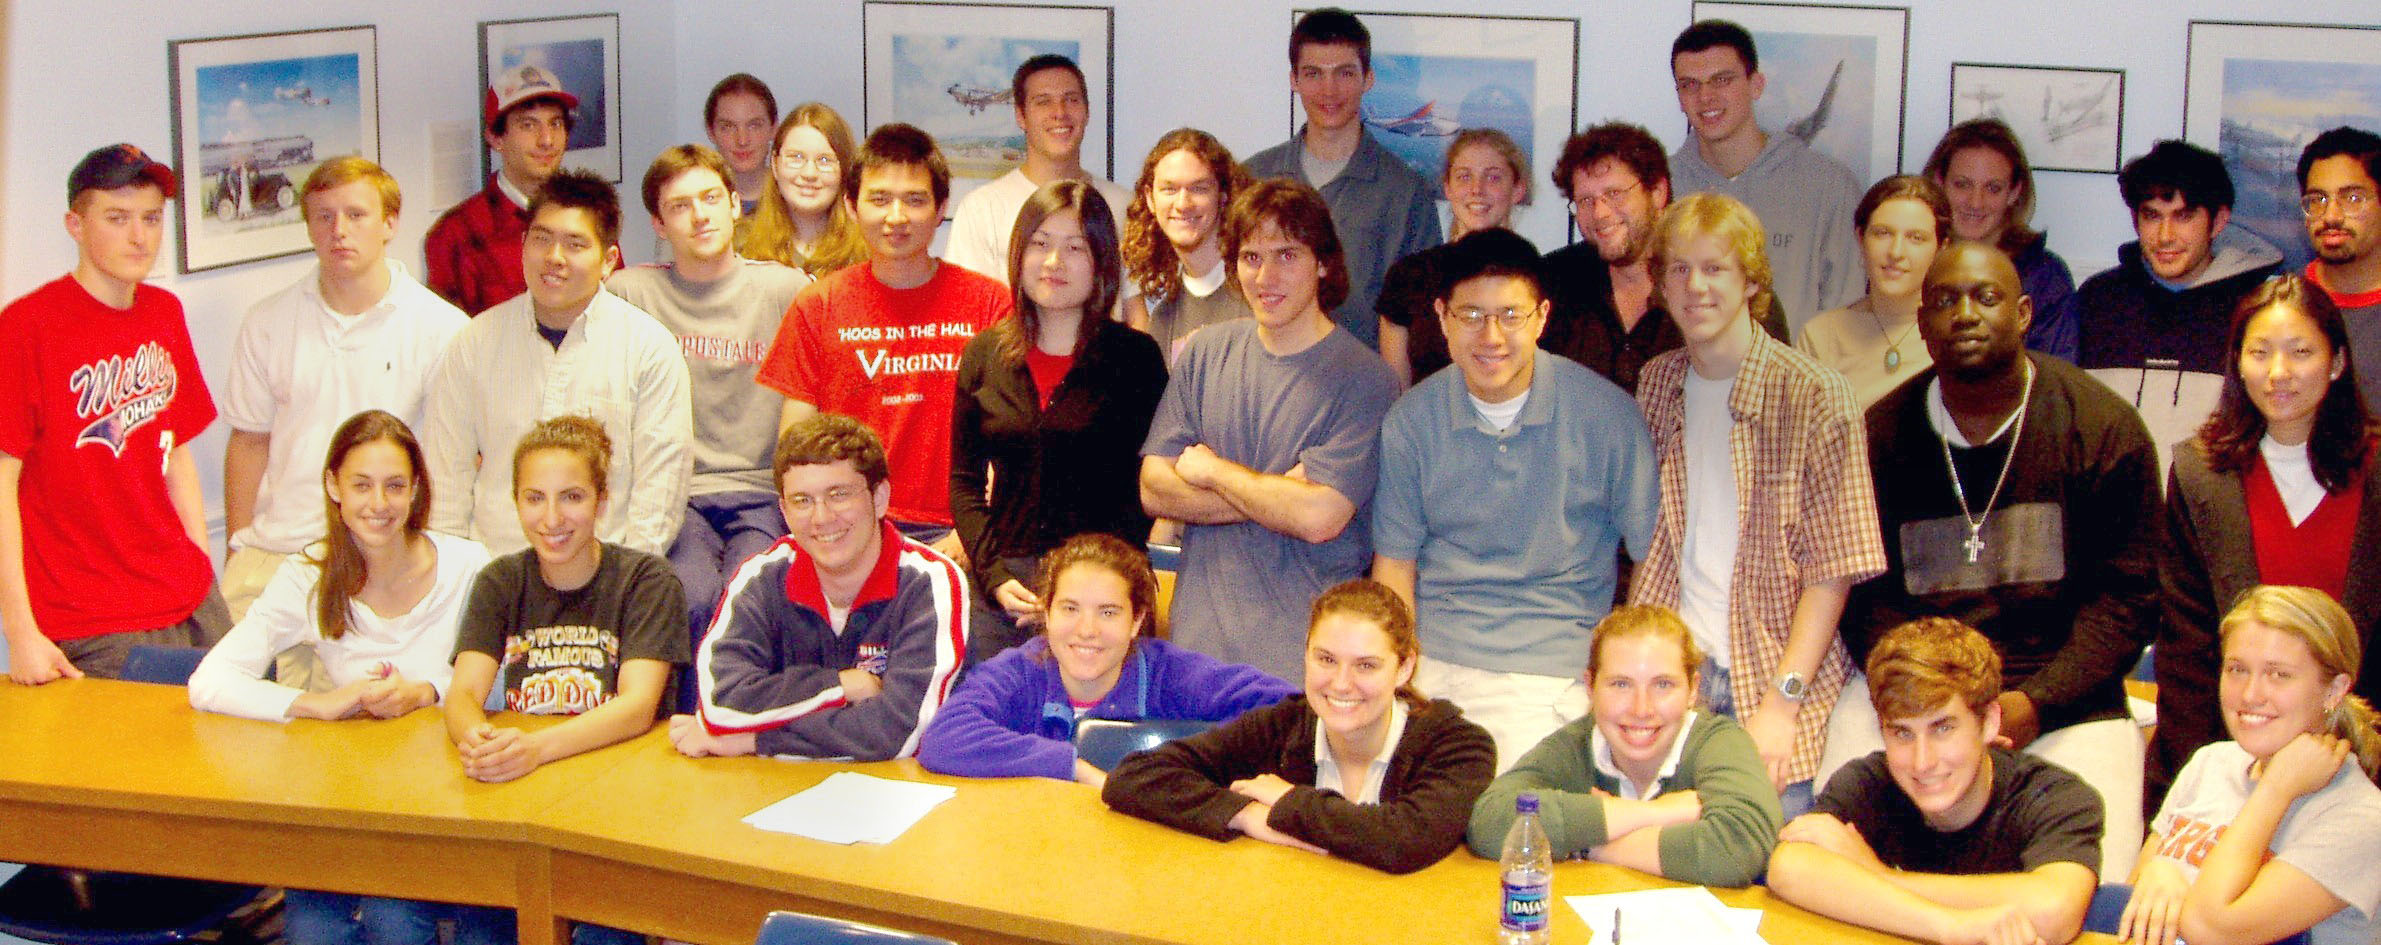
\includegraphics[width=4.3in]{images/cs200-spring2003-edited.jpg}
\newline{\bf Spring 2003}
\end{center}

\begin{minipage}[c]{2.7in}
\center
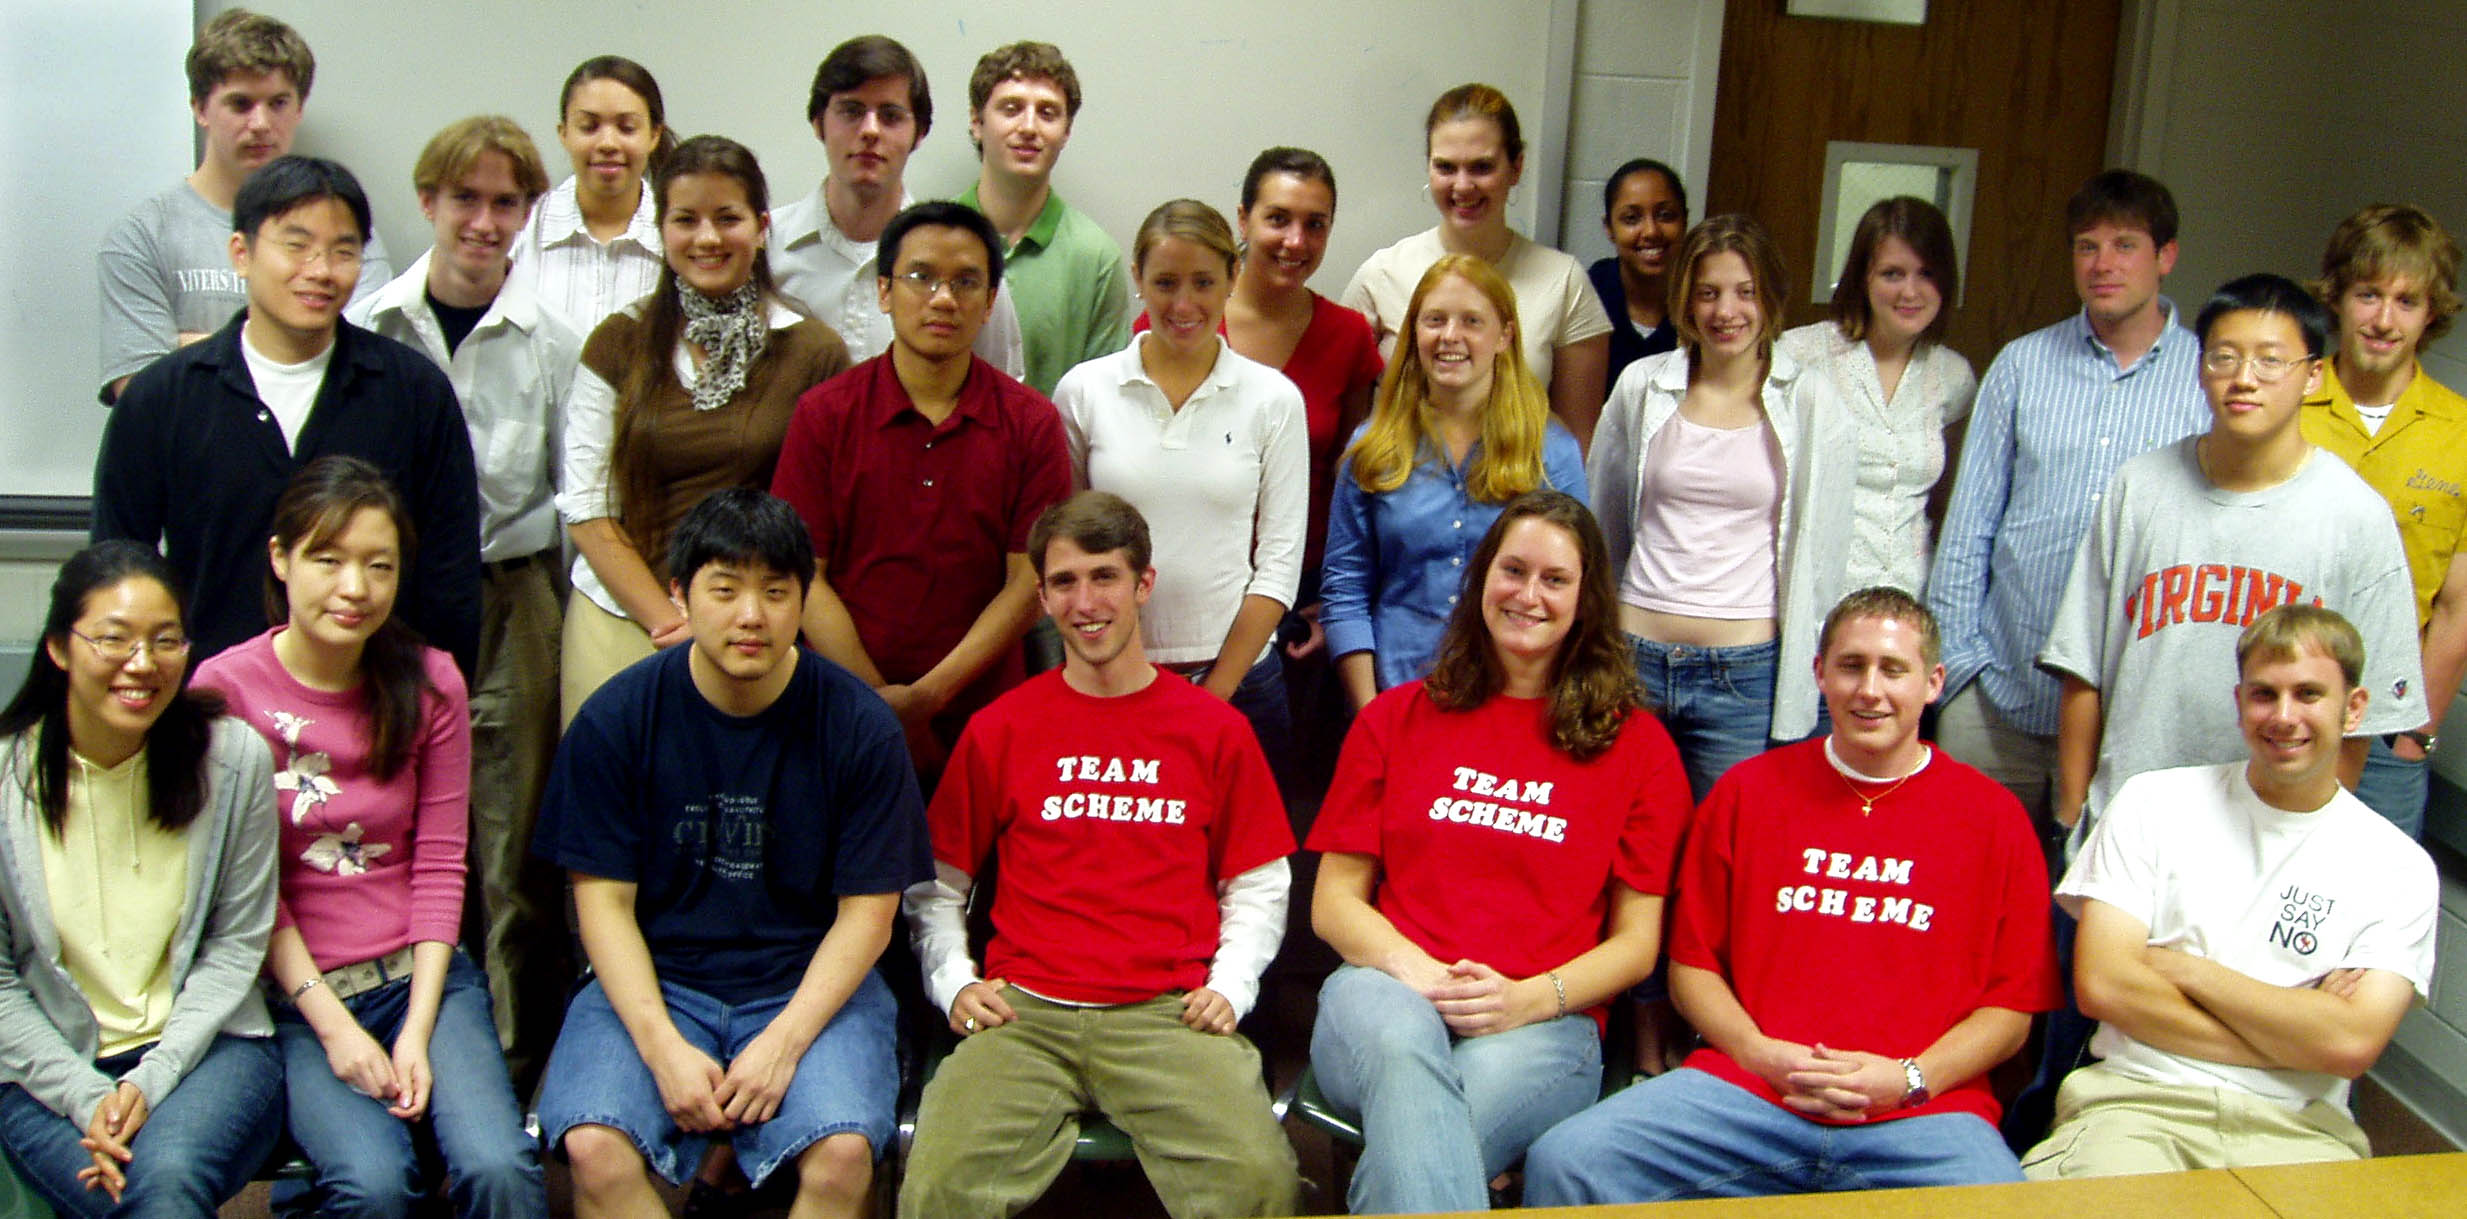
\includegraphics[height=1.45in]{images/cs200-spring2004-edited.jpg}
\newline{\bf Spring 2004}
\end{minipage}
\quad
\begin{minipage}[c]{2.4in}
\center
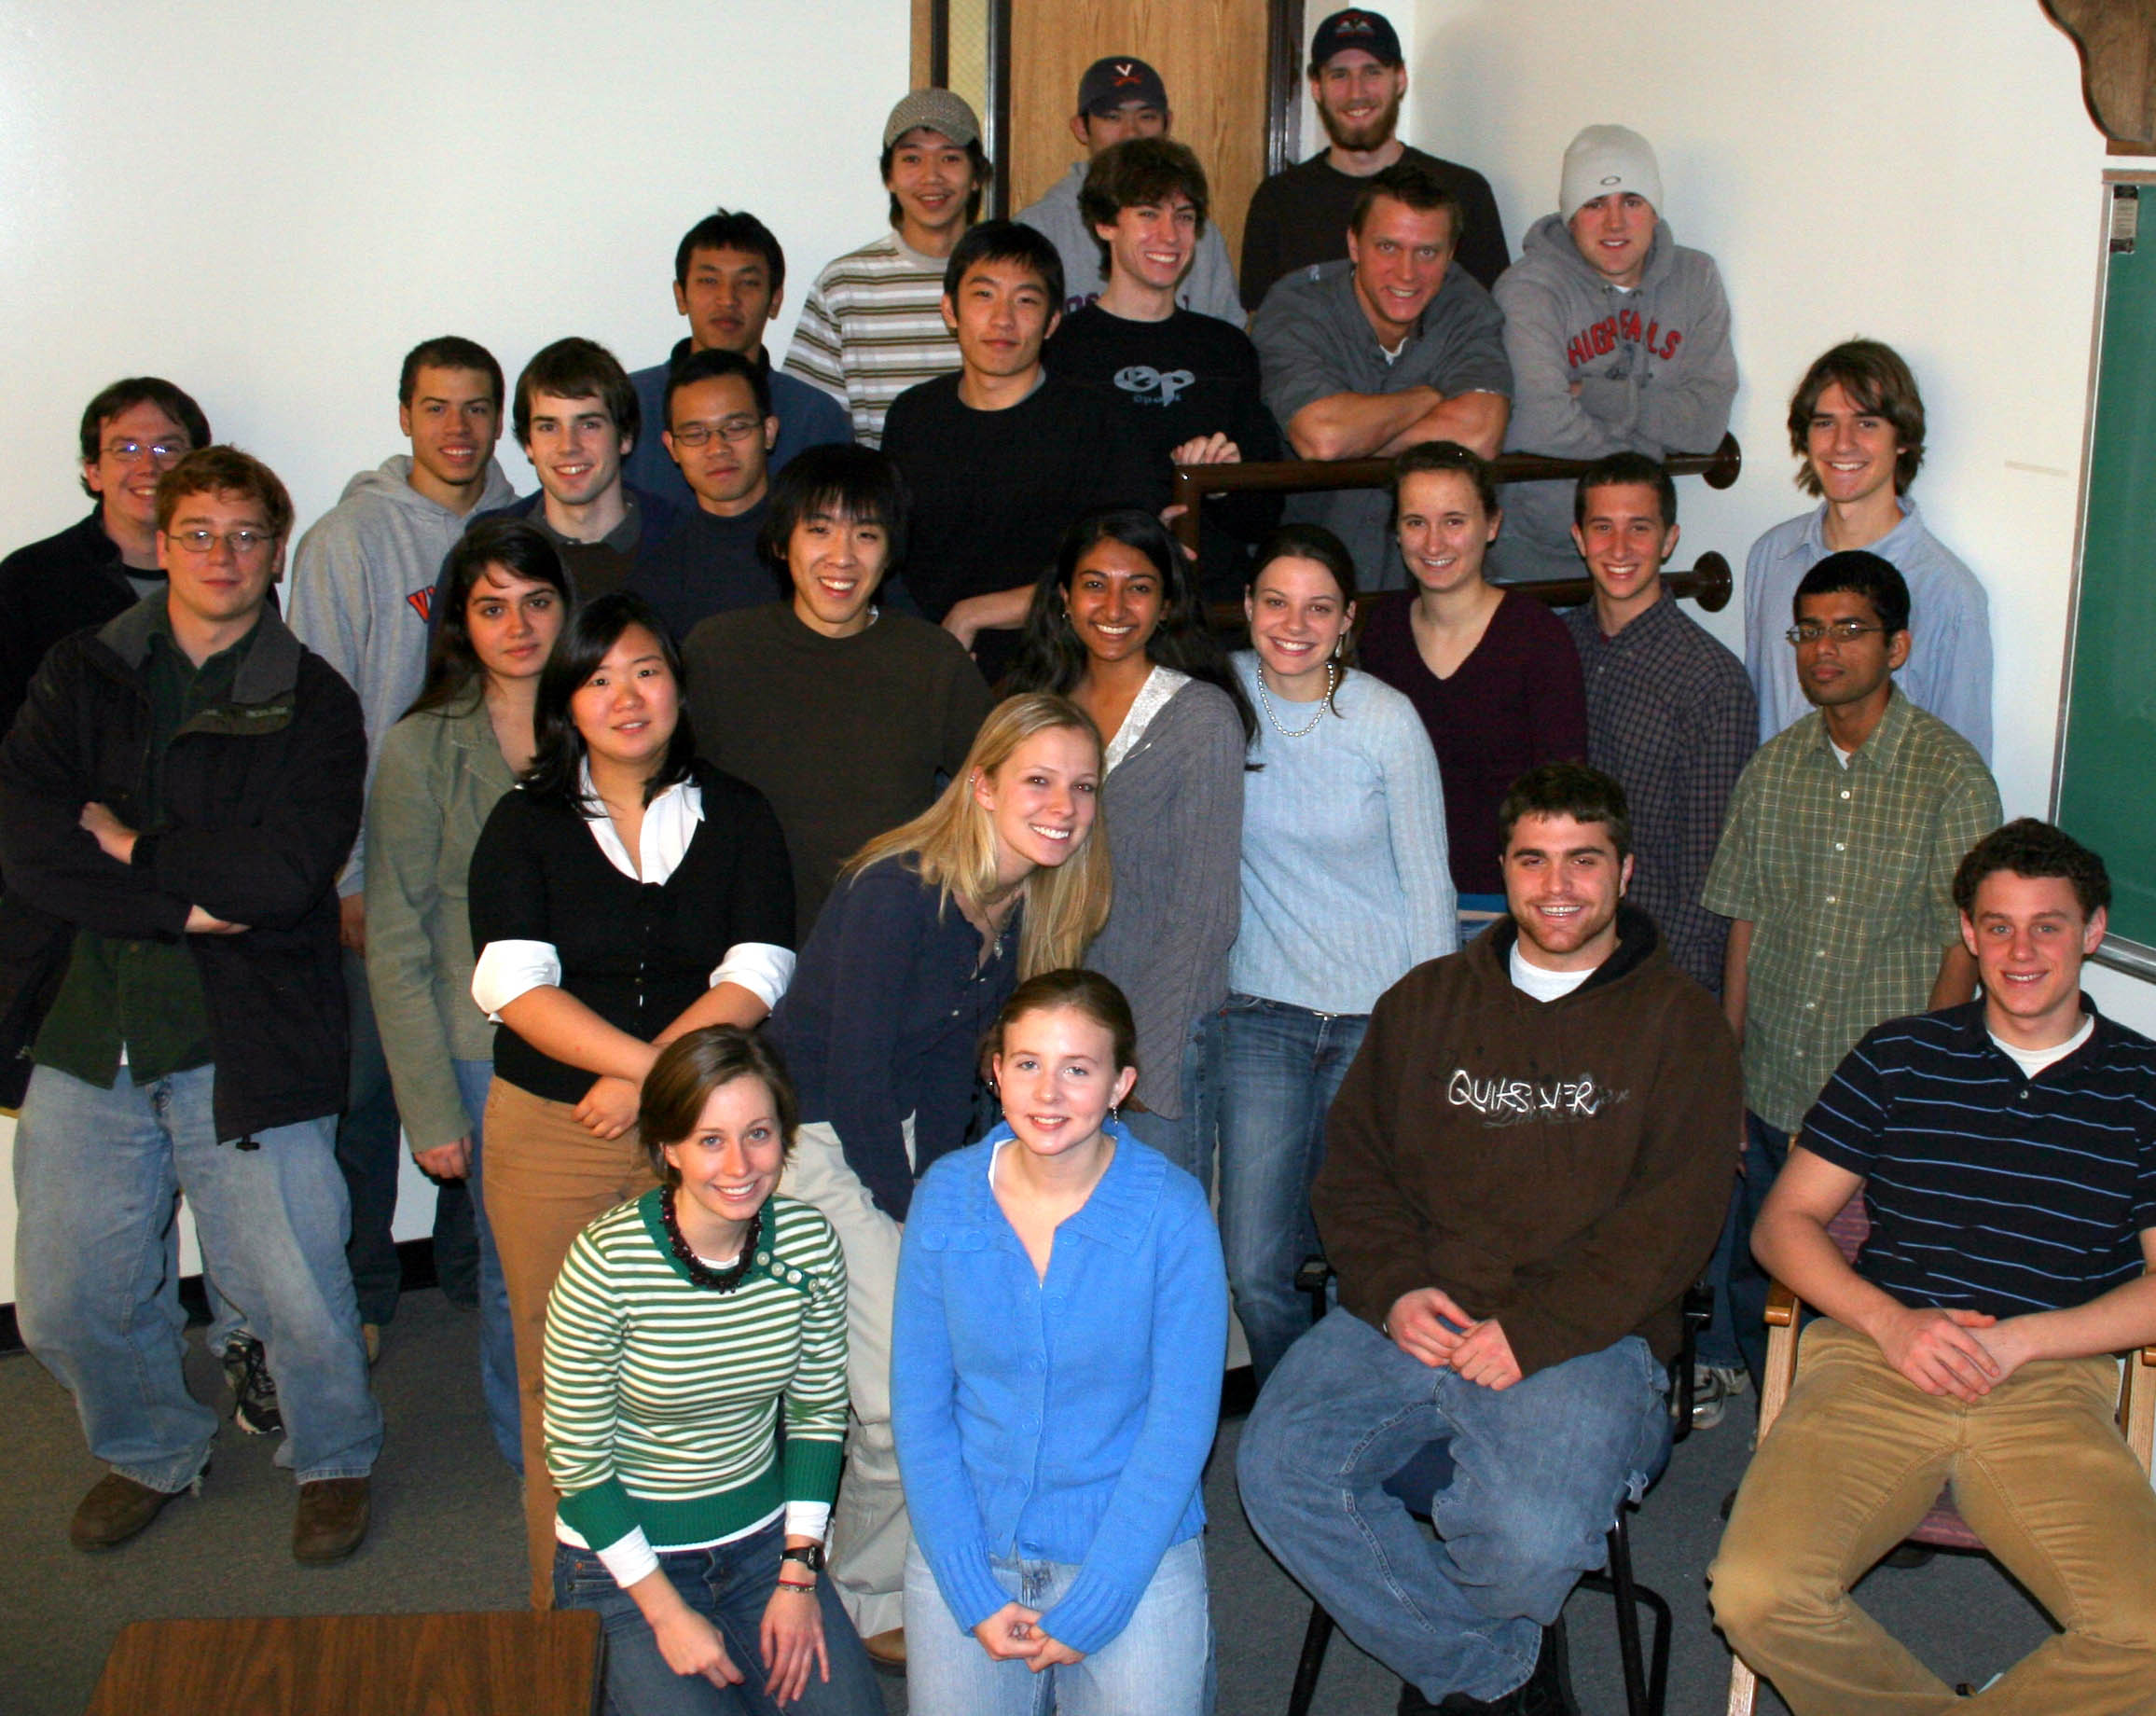
\includegraphics[height=1.45in]{images/cs150-fall2005-edited.jpg}
\newline{\bf Spring 2005}
\end{minipage}
